\section{Matching games}\label{sec:matching}

The primary motivation for this work is to move away from the greedy approaches
defined above by incorporating some techniques from game theory, namely:
matching games. The purpose of solving a matching game is to link the elements
of two sets in a `fair' way so that no element could feasibly be better off. By
considering the virtual modes found during Huang's method with some suitable
subset of our dataset as a matching game to be solved, we hope to find a
closer-to-optimal set of initial modes for the \(k\)-modes algorithm.

\begin{definition}\label{def:matching_game}
    Consider two sets \(S, R\) each of size \(N\), and let us call them 
    `suitors' and `reviewers'. Each element of \(S\) and \(R\) has associated 
    with it a preference list of the other set's elements. These preference 
    lists are ranked in descending order. We consider the preference lists as 
    functions which produce tuples, \(f\) and \(g\) respectively:
	\[
	    f : S \to R^n, \ g : R \to S^n
	\]
	This construction of sets and preference lists is called a 
    \emph{matching game} of size \(N\) and we denote the game itself by 
    \((S,R)\).
	
    A matching, \(M\), is defined to be any bijection between \(S\) and \(R\). 
    If \(s \in S\) and \(r \in R\) are matched by \(M\), then we write
    \(M(s)~=~r\). A matching \(M\) is considered to be either stable or unstable
    based on the preference lists of its suitors and reviewers, and the presence
    of blocking pairs.
\end{definition}

\begin{definition}\label{def:blocking_pair}
    Let \((S, R)\) be a matching game of size \(N\) with some matching \(M\). A 
    pair \((s, r) \in S \times R\) is said to \emph{block} \(M\) if \(M(s) \neq
    r\) but \(s\) prefers \(r\) to \(M(s) = r'\) and \(r\) prefers \(s\) to
    \(M^{-1}(r) = s'\). That is, \(r\) appears before \(r'\) in \(f(s)\) and
    \(s\) appears before \(s'\) in \(g(r)\).
\end{definition}

\begin{definition}\label{def:stable_matching}
    Let \((S, R)\) be a matching game of size \(N\) with some matching \(M\). 
    Then we say \(M\) is a \emph{stable matching} if there are no blocking 
    pairs, and \emph{unstable} otherwise.
\end{definition}

%\begin{example}\label{example:matching}
    Consider the following example with \(S = \{A, B, C\}\) and \(R = \{D, E,
    F\}\). We can visualise this matching game as a bipartite graph as in
    Figure~\ref{fig:matching_bipartite}. In this representation, an edge between
    two vertices indicates that they are matched by \(M\). Beside each node is 
    the name of the node and a complete ranking of its complementary set's 
    elements. We interpret these rankings as the values of our preference list 
    functions. Here, for instance, \(A\) would most prefer to be matched with 
    \(D\), then \(E\), and finally \(F\).
    
    \begin{figure}[h]
        \centering
        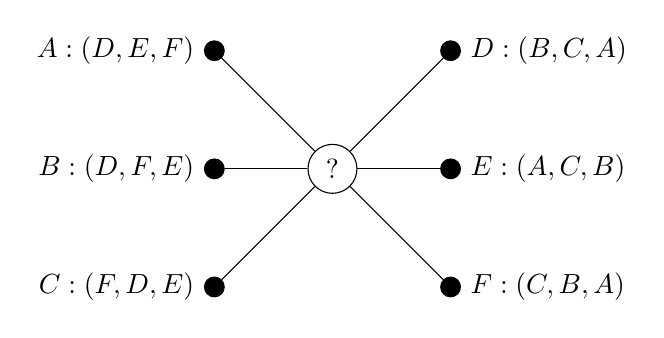
\begin{tikzpicture}[scale=0.5]

    % Suitors
    \node[draw, shape=circle, fill, inner sep=0, minimum size=0.25cm,
    label=left: {\(A: (D, E, F)\)}] (A) at (0, 0) {};
    \node[draw, shape=circle, fill, inner sep=0, minimum size=0.25cm, 
    label=left: {\(B: (D, F, E)\)}] (B) at (0, -3) {}; 
    \node[draw, shape=circle, fill, inner sep=0, minimum size=0.25cm, 
    label=left: {\(C: (F, D, E)\)}] (C) at (0, -6) {};

    % Reviewers
    \node[draw, shape=circle, fill, inner sep=0, minimum size=0.25cm, 
    label=right: {\(D: (B, C, A)\)}] (D) at (6, 0) {};
    \node[draw, shape=circle, fill, inner sep=0, minimum size=0.25cm, 
    label=right: {\(E: (A, C, B)\)}] (E) at (6, -3) {};
    \node[draw, shape=circle, fill, inner sep=0, minimum size=0.25cm,
    label=right: {\(F: (C, B, A)\)}] (F) at (6, -6) {};

    % Question mark node
    \node[draw, shape=circle] (q) at (3, -3) {?};
        
    % Lines into (?)
    \foreach \x in {A, B, C, D, E, F}
        \draw (\x) -- (q);

\end{tikzpicture}
\caption{A simple matching game represented on a bipartite
    graph.}\label{fig:matching_bipartite}

    \end{figure}

    Suppose we have the matching shown in Figure~\ref{fig:unstable_matching} for
    our game. This matching, \(M\) is valid since it is a bijection between 
    \(S\) and \(R\) but it is not stable. For instance, we have \((B, D)\) as a
    blocking pair since \(B\) would rather be matched with \(D\) than its 
    current match \(E\), and \(D\) would prefer to be matched with \(B\) than
    its current match \(A\).

    \begin{figure}[h]
        \centering
        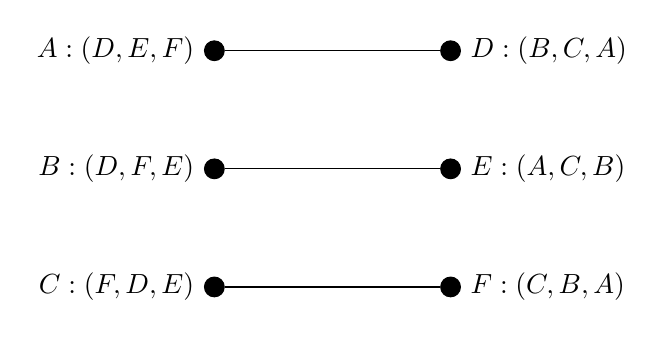
\begin{tikzpicture}[scale=0.5]

    % Suitors
    \node[draw, shape=circle, fill, inner sep=0, minimum size=0.25cm, 
    label=left: {\(A: (D, E, F)\)}] (A) at (0, 0) {};
    \node[draw, shape=circle, fill, inner sep=0, minimum size=0.25cm, 
    label=left: {\(B: (D, F, E)\)}] (B) at (0, -3) {}; 
    \node[draw, shape=circle, fill, inner sep=0, minimum size=0.25cm, 
    label=left: {\(C: (F, D, E)\)}] (C) at (0, -6) {};

    % Reviewers
    \node[draw, shape=circle, fill, inner sep=0, minimum size=0.25cm, 
    label=right: {\(D: (B, C, A)\)}] (D) at (6, 0) {};
    \node[draw, shape=circle, fill, inner sep=0, minimum size=0.25cm, 
    label=right: {\(E: (A, C, B)\)}] (E) at (6, -3) {};
    \node[draw, shape=circle, fill, inner sep=0, minimum size=0.25cm,
    label=right: {\(F: (C, B, A)\)}] (F) at (6, -6) {};

    % Lines
    \draw (A) -- (D);
    \draw (B) -- (E);
    \draw (C) -- (F);

\end{tikzpicture}
\caption{A example of an unstable matching for our
    game.}\label{fig:unstable_matching}

    \end{figure}

    We can make this matching stable by switching these pairs as in
    Figure~\ref{fig:stable_matching}. Here we have that each suitor is matched 
    with their most preferred reviewer so as not to form a blocking pair. We 
    call such a matching \emph{suitor-optimal}.

    \begin{figure}[h]
        \centering
        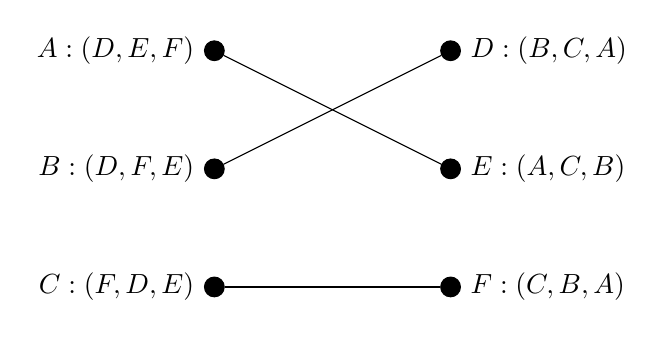
\begin{tikzpicture}[scale=0.5]

    % Suitors
    \node[draw, shape=circle, fill, inner sep=0, minimum size=0.25cm, 
    label=left: {\(A: (D, E, F)\)}] (A) at (0, 0) {};
    \node[draw, shape=circle, fill, inner sep=0, minimum size=0.25cm, 
    label=left: {\(B: (D, F, E)\)}] (B) at (0, -3) {}; 
    \node[draw, shape=circle, fill, inner sep=0, minimum size=0.25cm, 
    label=left: {\(C: (F, D, E)\)}] (C) at (0, -6) {};

    % Reviewers
    \node[draw, shape=circle, fill, inner sep=0, minimum size=0.25cm, 
    label=right: {\(D: (B, C, A)\)}] (D) at (6, 0) {};
    \node[draw, shape=circle, fill, inner sep=0, minimum size=0.25cm, 
    label=right: {\(E: (A, C, B)\)}] (E) at (6, -3) {};
    \node[draw, shape=circle, fill, inner sep=0, minimum size=0.25cm,
    label=right: {\(F: (C, B, A)\)}] (F) at (6, -6) {};

    % Lines
    \draw (A) -- (E);
    \draw (B) -- (D);
    \draw (C) -- (F);

\end{tikzpicture}
\caption{An example of a stable matching for our
    game.}\label{fig:stable_matching}

    \end{figure}
\end{example}


\subsection{The Gale-Shapley algorithm}\label{subsec:galeshapley}

The Gale-Shapley algorithm is known to find a unique stable matching for any 
matching game of size \(N\). This matching is also considered to be 
suitor-optimal. That is, each suitor is matched with the best possible reviewer
that ensures a stable matching, but is in fact the worst possible matching for 
the reviewers. \textcolor{red}{[cite or have these theorems stated/proven]} 

As was discussed at the start of Section~\ref{sec:matching}, the outline of
the method proposed in this paper is to extend Huang's method by considering the
virtual modes with some subset of the data as a matching game to be solved. It
should be noted, however, that in this method we may not have equally sized 
sets of suitors and reviewers. As a result of this, the Gale-Shapley algorithm 
becomes inapplicable as the matching produced \(M\) would not be a bijection of 
our suitors and reviewers.

\subsection{The capacitated Gale-Shapley algorithm for the hospital-resident 
	problem}\label{subsec:capacitated_galeshapley}

The situation where a large set of suitors are to be matched with a number
reviewers is not limited to abstraction. A practical example of this problem is
how to best assign a cohort of medical students to a group of hospitals. Here, 
we have all of the requisite components of a matching game:

\begin{itemize}
	\item A set of reviewers (the hospitals) and a set of suitors (the potential
        residents) 
	\item A ranking of the students/residents by the hospitals, and vice versa
\end{itemize}

The only obstacle which stops us from using the Gale-Shapley algorithm is the 
disparity in the sizes of our sets. In reality, hospitals need not always take 
at most one resident on from a cohort of medical students. So each hospital has
a capacity associated with it and we can consider our matching game to be
`capacitated'. By this we mean that each reviewer (hospital) may be matched with
any number of suitors (students) up to their capacity, making our matching
\(M:~S~\to~R\) surjective.

Research surrounding the hospital-resident assignment problem is well-documented 
\textcolor{red}{[cite]} and an extension of the Gale-Shapley algorithm was
developed to solve it, awarding the authors the 2012 Nobel Prize in Economic
Sciences. This algorithm is currently used by the National Resident Matching
Program (\url{http://www.nrmp.org}) to assign medical students to hospitals in
the United States of America.

As before, we consider a set of suitors and reviewers denoted by \(S\) and 
\(R\). These sets are no longer (necessarily) the same size. We also have our 
preference lists \(f, g\), and a set \(C = \{c_1, \ldots, c_{|R|}\}\) of 
reviewer capacities. Finally, let \(S_u \subset S\) denote the set of suitors 
that are currently unmatched. The capacitated Gale-Shapley algorithm is given 
below.

\begin{singlespace}
    \begin{algorithm}[H]
\caption{Capacitated Gale-Shapley}\label{alg:cap-galeshapley}
    \begin{algorithmic}[0]
        \State{\textbf{Input:} two sets of objects \(S, R\), a set of capacities
        for the elements of \(R\), denoted by
        \(C~=~\left\{c_1,~\ldots,~c_{|R|}\right\}\), and two preference list
        functions, \(f, g\)}
        \State{\textbf{Output:} a surjective matching \(M\) between \(S\) and
        \(R\)\\}
        \\
        \Comment{Initialise all suitors and reviewers to be unmatched}
        \For{\(s \in S\)}
            \State{\(M(s) \gets \emptyset\)}
	    \EndFor%
        \For{\(r \in R\)}
            \State{\(M^{-1}(r) \gets \emptyset\)}
	    \EndFor%
        \State{\(S_u \gets S\)}
        \\
        \\
        \Comment{Find a tentative match for some currently unmatched suitor}
        \While{\(|S_u| > 0\)}
            \State{Select any \(s \in S_u\).}
            \If{\(|f(s)| = 0\)}
                \State{\(S_u \gets S_u \setminus \{s\}\)}
		    \Else%
                \State{Select \(s\)'s most preferred reviewer \(r \in R\).}
                \\
                \Comment{If \(r\) has room, match to \(s\)}
                \If{\(|M(r)| < c_r\)}
                    \State{\(M(r) \gets M(r) \cup \{s\}\)}
                    \State{\(S_u \gets S_u \setminus \{s\}\)}
		        \Else%
                \\
                \Comment{Otherwise determine whether their matching would be
                preferable to \(r\) over its worst current matching}
                    \State{Find \(s' \in M(r)\) such that \(r\) prefers \(s'\)
                    least.}
                    \If{\(r\) prefers \(s\) to \(s'\)}
                        \State{\(M(r) \gets M(r) \cup \{s\}\)}
                        \State{\(S_u \gets S_u \cup \{s\}\)}
                        \State{\(M(r) \gets M(r) \setminus \{s'\}\)}
                        \State{\(S_u \gets S_u \cup \{s'\}\)}
				    \Else%
                        \State{\(f(s) \gets f(s) \setminus \{r\}\)}
		            \EndIf%
                \EndIf%
		    \EndIf%
	    \EndWhile%
	\end{algorithmic}
\end{algorithm}

\end{singlespace}
